Introducing STM as a electronically sensitive scanning probe method, the atomic force microscopy is another scanning probe tool. To scan the surface of the sample, one uses an small tip to interact with it on short distance where forces between sample and tip occur. The force induced movement of the tip is then interpreted and information about the surface may be derived. If the tip interacts with the sample, its oscillation is hindered/amplified and the frequency of the oscillation shifts. From this shift one can estimate the strength of the acting force. Since every type of adsorbate atom acts in different ways with the tip, AFM is element specific. When the tunneling current through the AFM tip is recorded, simultaneous AFM and STM measurements are possible. 
\subsection{Theory}

\begin{figure}\centering
	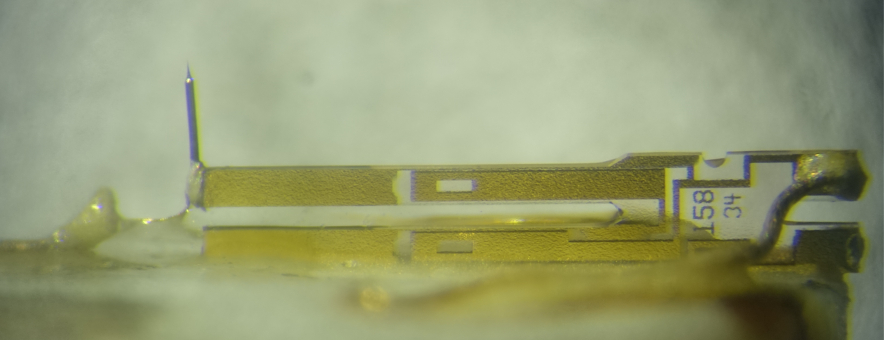
\includegraphics[width=0.7\textwidth]{./images/AFM-qplus-photograph}
	\caption{Photograph of the tuning fork and cantilever. The tip is glued to the tuning fork on the left side. From \cite{he_bottom-up_2017}}
\label{fig:AFM-tuning-fork}
\end{figure}	

\begin{figure}\centering
	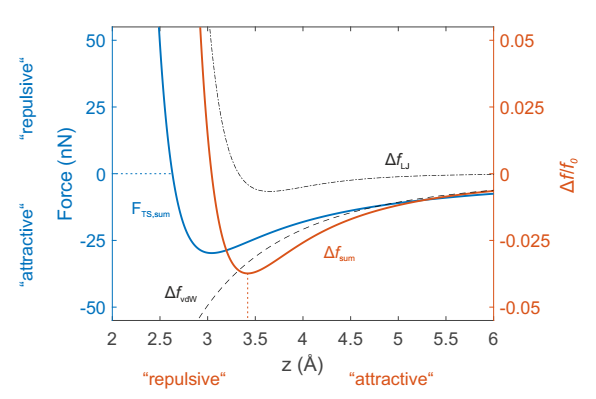
\includegraphics[width=0.7\textwidth]{./images/AFM-graph-martin}
		\label{fig:AFM-force}
\caption{Sketch of tip-sample interaction force (blue) together with relative frequency shift. Contributions of vdW and Lennard Jones like forces result in two separable frequency shifts $\Delta f_{LJ}$ and $\Delta f_{vdW}$ (black) that add up to a total of $\Delta f_{sum}$ (orange) from where the total force is derived. From \cite{schwarz_assembly_2018}}
\label{fig:AFM-sketch}%
\end{figure}

Amongst others, forces between AFM tip and sample are made up of attractive forces like van der Waals forces and repulsive forces like mechanical contact force and pauli repulsion.

\begin{itemize}
 \item Van-der-waals interaction (always attractive)
 $$ F_{vdW} = - \frac{A_HR}{6z^2}$$
 \item Mechanical contact force, Pauli repulsion and chemical bonding are modeled in the Lennard Jones Potential
$$ F_{LJ} = - \frac{12 E_{min}}{z_0} \left ( \left (\frac{z_0}{z} \right ) ^{13} - \left ( \frac{z_0}{z} \right )^7 \right ) $$
\end{itemize}

The typical resulting force between tip and sample is artistically shown in \autoref{fig:AFM-sketch}. On the top part a tuning fork with an atomic tip is shown on top of the sample surface. The interaction forces $F_{ts}$ act between tip and sample and are indicated by an arrow. In the lower part a representation of the resulting force in dependence of the tip-sample distance is shown. Although many different forces may act, the resulting potential is often modeled with a Lennard-Jones-Potential ($LJ$)\cite{jones_determination_1924}. Two of these are plotted with green and blue dots. The attractive vdW force is plotted in dashed green. The sum of the acting forces is labeled $\sum$. A typical frequency shift $\Delta f$ is given as red graph. 

$$\Delta f = - \frac{f_0}{2k_0}\frac{\delta F_{TS}}{\delta z}$$

One can distinguish different regimes as indicated by the arrows. When tip and sample are in considerable distance to each other, the attractive vdW forces are the dominant part in the sum. While the tip approaches the sample, more and more interactions with the surface and adsorbate add to this force, strengthening $F_{ts}$. When the separation reaches $z_0$, the distance becomes so small that repulsive forces overcome the attractive one - entering the repulsive regime shortly afterwards. \textcolor{red}{\textbf{The best images were recorded close to the onset where $F_{ts}$ becomes repulsive.}}

AFM is used here in the non-contact mode (\textbf{nc-mode}): The tuning fork is driven at its resonance frequency with fixed amplitude and at a certain distance to the sample. Long-range forces like van-der-waals and others change the resonance frequency of the cantilever. This change is a indication of the acting force between cantilever and sample. 

\textcolor{red}{\textbf{AFM measures a true height-profile of the sample (and not a mix of electronic and geometric information projected onto a 2D-map like in STM). Contour lines in $\Delta f$ images represent lines with the same tip interaction strength.}}

To increase the resolution the tip can be functionalized with CO. This method is widely used\footnote{Only a few examples from the recent years can be found here \cite{albrecht_direct_2016, kawai_multiple_2018, kawai_atomically_2015, schulz_elemental_2018, gross_chemical_2009, pavlicek_generation_2017, schwarz_corrugation_2017}} to investigate not only geometric features that are not directly accessible in STM, but also chemical differences on the sample\cite{wang_exploration_2017}.

\subsection{\textcolor{red}{\textbf{Experimental details}}}
The used LT-AFM features a tuning fork sensor, as shown in \autoref{fig:AFM-tuning-fork}. Here the tip is positioned on below an oscillating fork that is operated close to its resonance frequency $f_0$.  A piezo element that continuously stimulates oscillations in a quartz crystal is used to drive the forced oscillation of the tuning fork ($f_0$, $k_0$). To its end the AFM/STM tip is attached and follows the oscillation that is driven close to its resonance frequency with a fixed amplitude. Measurements are done in the frequency modulated mode, meaning that the shift in resonance frequency, by an amount $\Delta f$  proportional to the force acting, is recorded in constant height to show the proportional local force gradient. The image is created by raster scanning the surface.

\subsection{\textcolor{red}{\textbf{Methods}}}
\textbf{$\Delta f $ images} recorded 

\textbf{$\frac{\Delta F}{\Delta z}$} spectroscopy is used to highlight changes in the local contact potential.

%\subsection{\textcolor{red}{\textbf{Limitations}}}
%\begin{itemize}
%	\item Element specific measurements in $\Delta f / \Delta z$ spectroscopy require long measurement times and a very little drift.
%\end{itemize}